\chapter{Protótipos}
\label{chap:prototipo}

A Figura \ref{img:prototipo_de_papel_info_posto} mostra o protótipo de papel da tela de quando um usuário chegar à um posto de combustíveis, onde terá informações sobre o mesmo.
\begin{figure}[H]
    \centering
    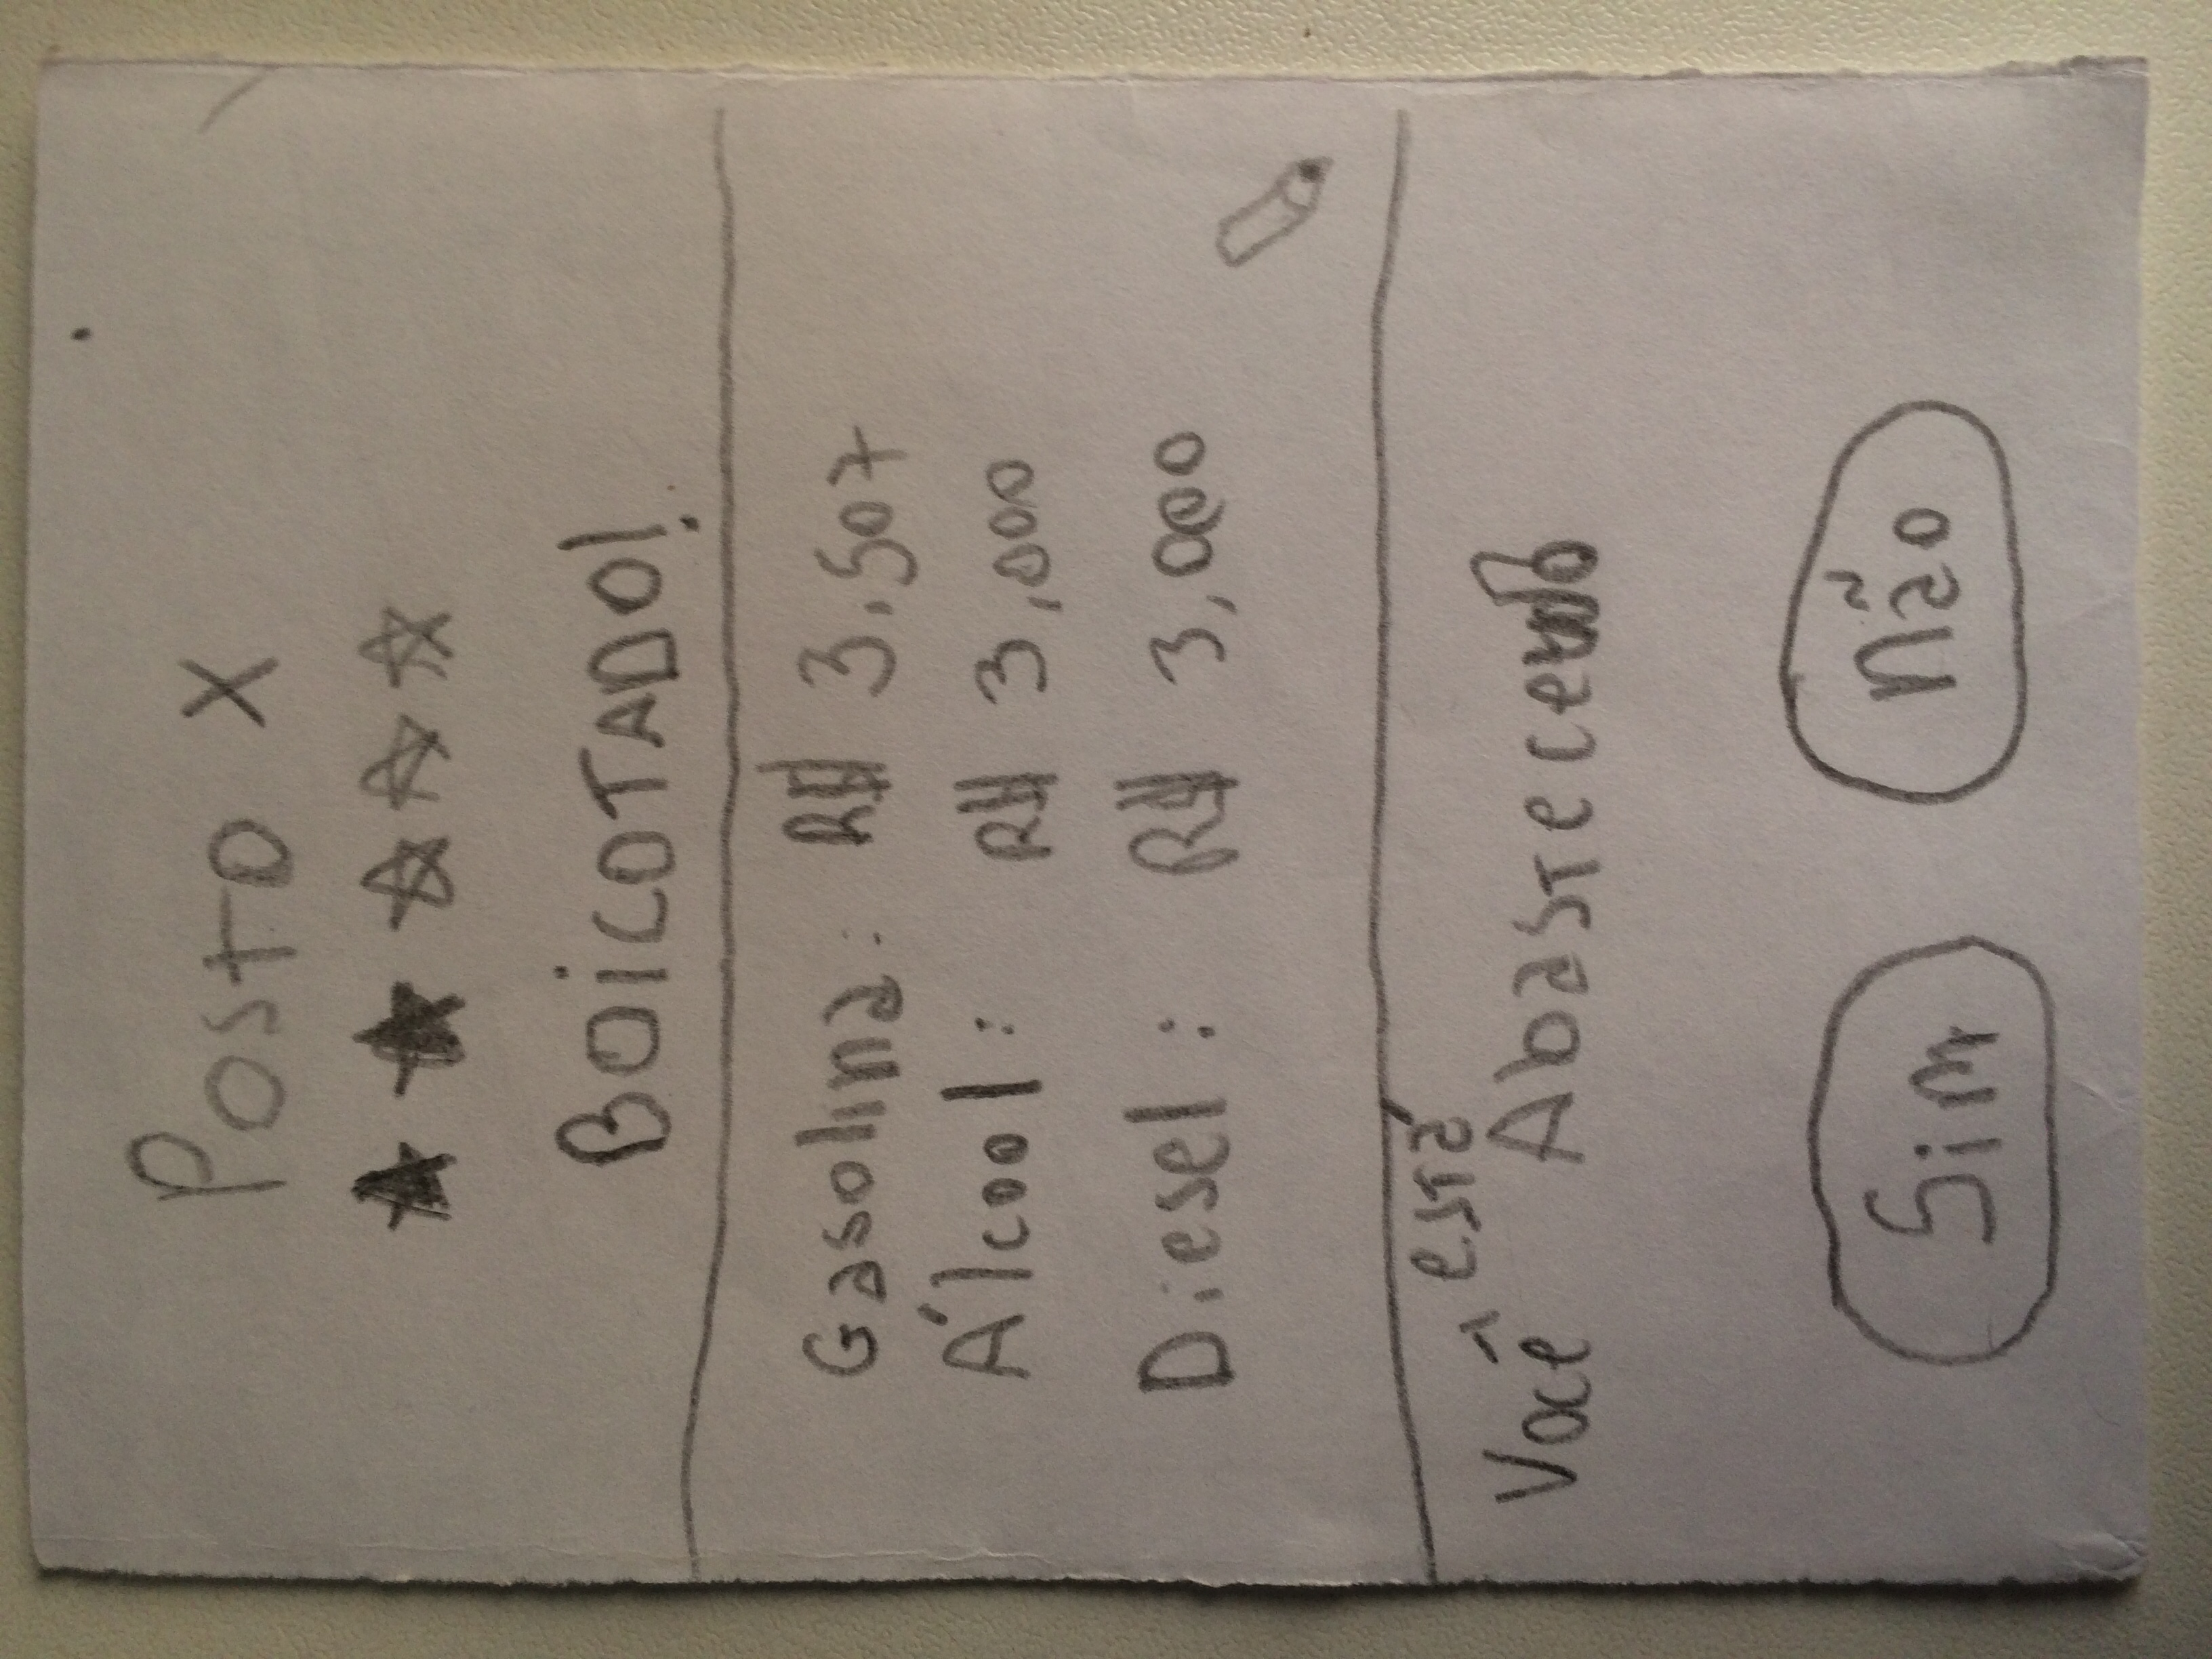
\includegraphics[scale=0.1, angle=-90]{figuras/prototipo_papel_info_posto.jpg}
    \caption[Protótipo de papel da tela de informações do posto]{Protótipo de papel da tela de informações do posto. Fonte: autores}
    \label{img:prototipo_de_papel_info_posto}
\end{figure}
 \pagebreak

A Figura \ref{img:prototipo_de_papel_precos_combustiveis} mostra o protótipo de papel de como será feito a avaliação dos preços dos combustíveis do posto que o usuário está localizado.
\begin{figure}[H]
    \centering
    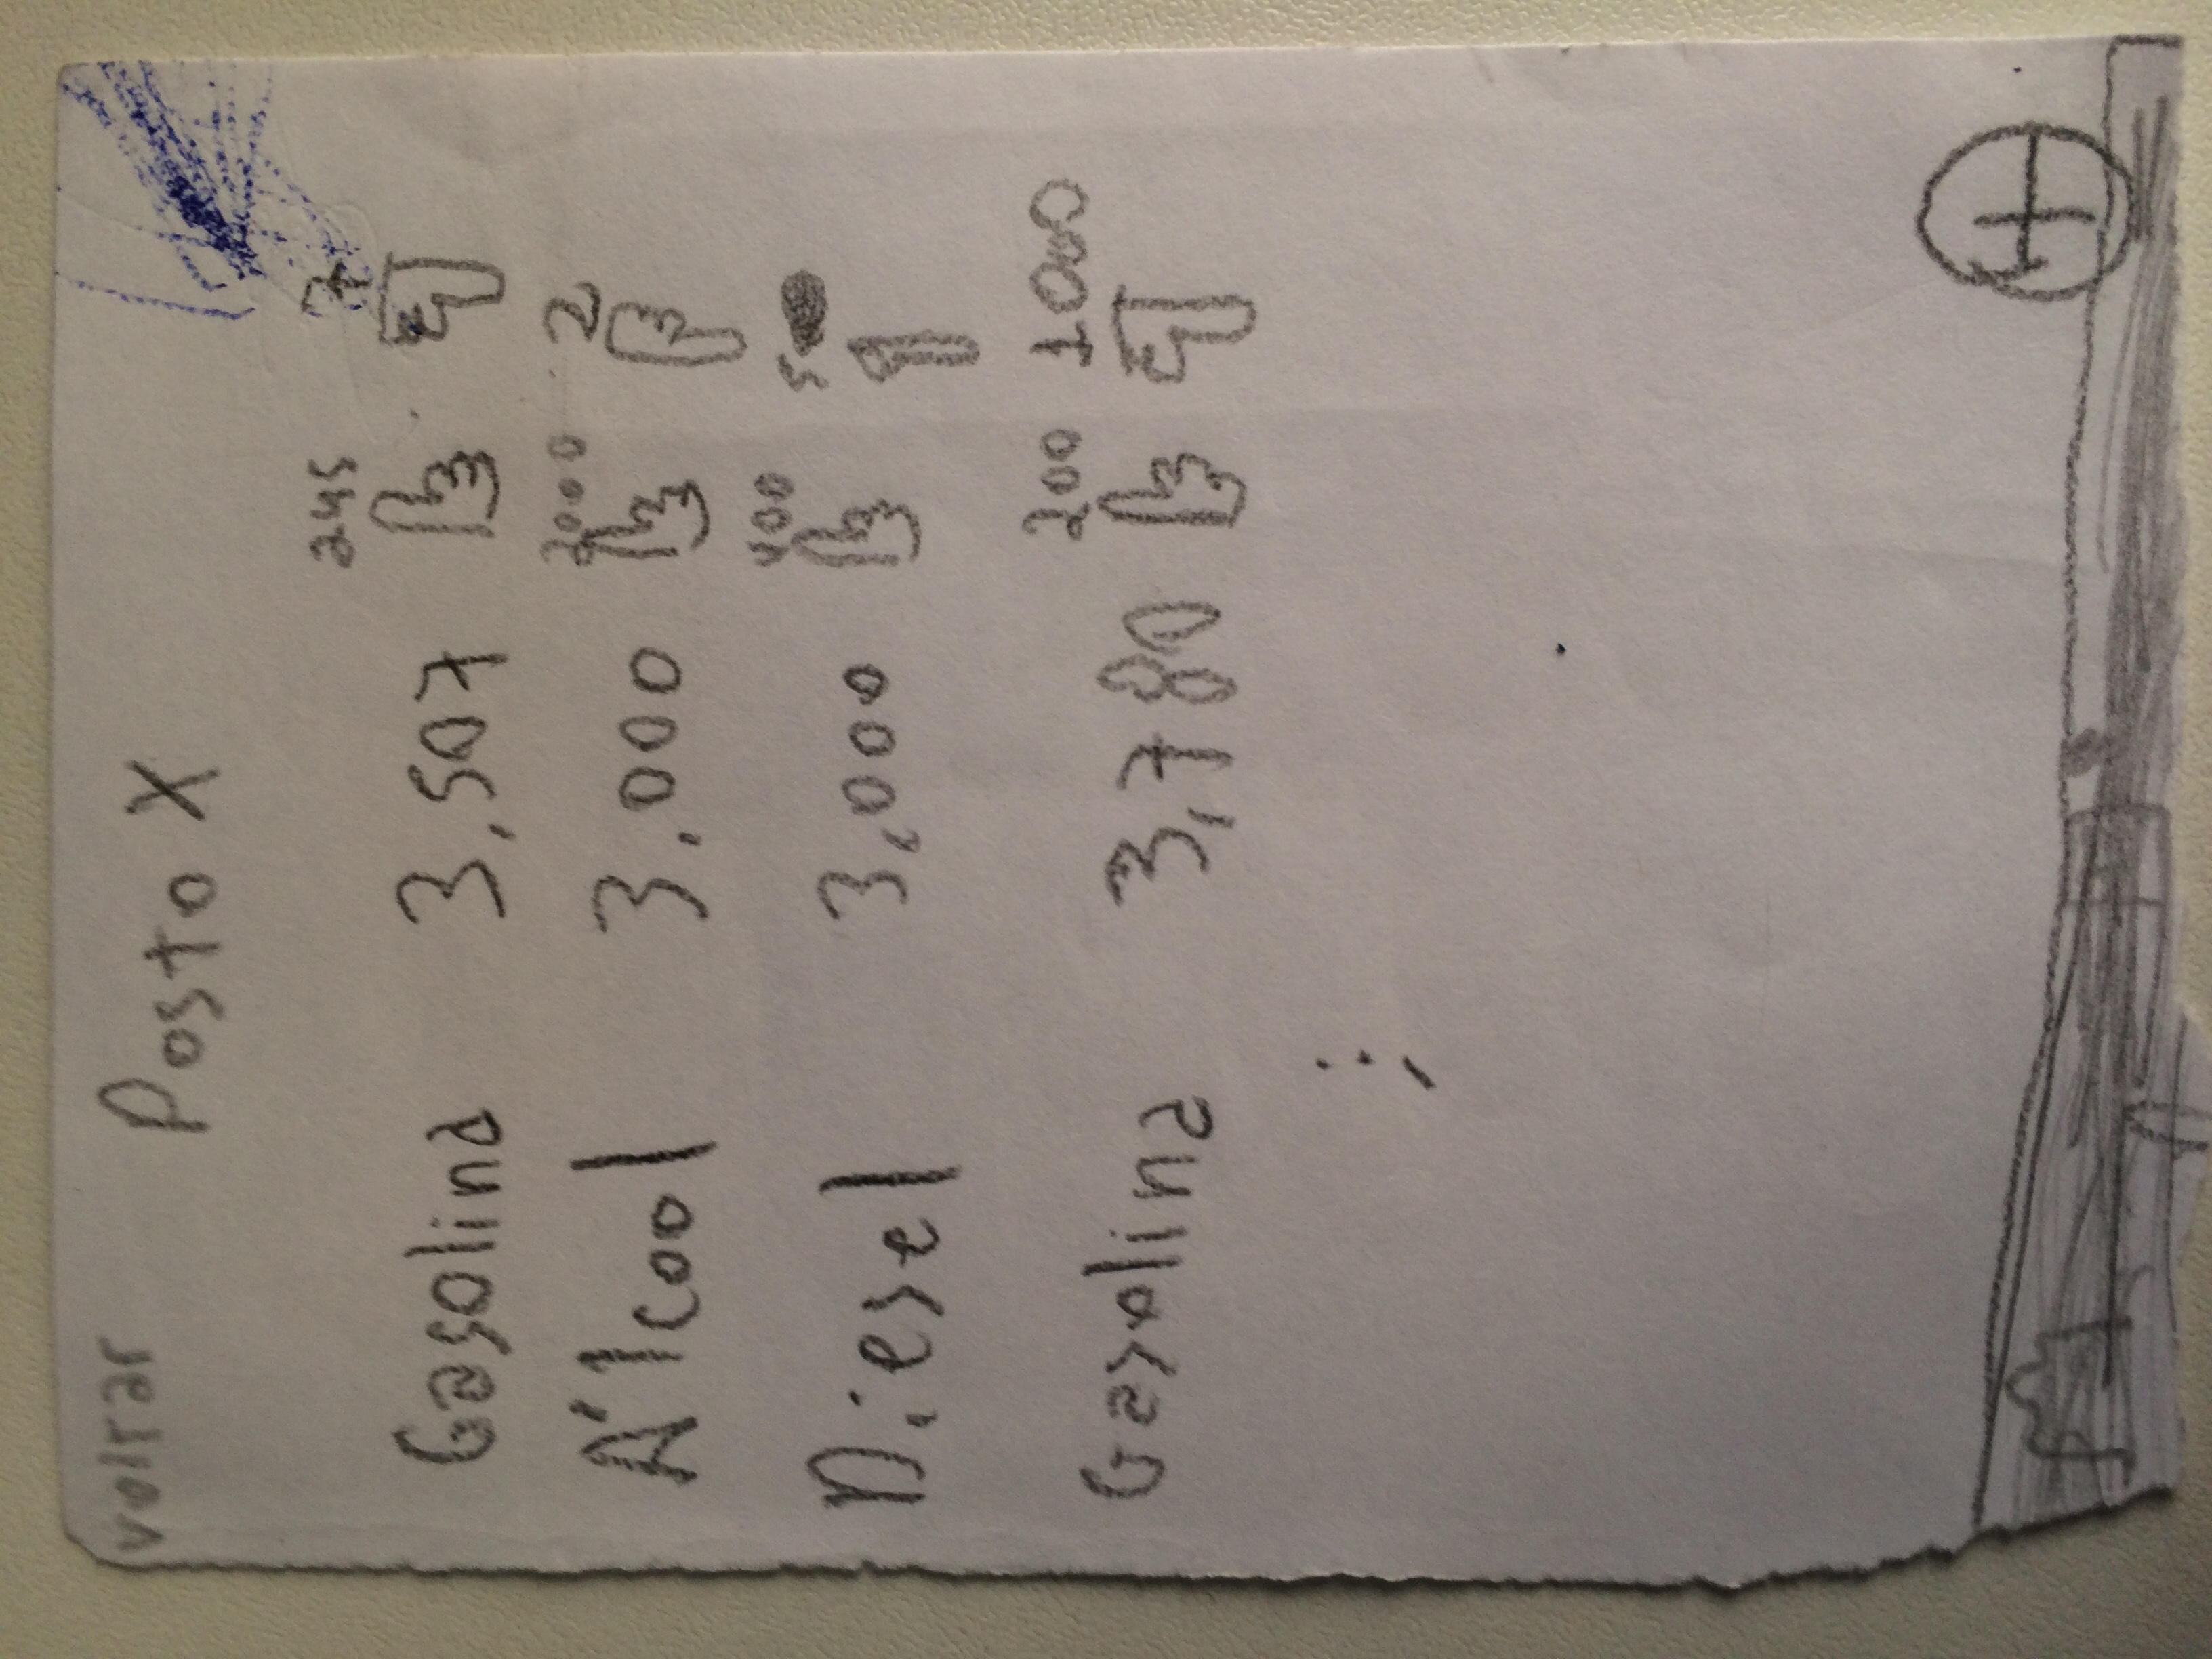
\includegraphics[scale=0.1, angle=-90]{figuras/prototipo_papel_avaliar_precos_postos.jpg}
    \caption[Protótipo de papel da tela de avaliar preço dos combustíveis]{Protótipo de papel da tela de avaliar preço dos combustíveis. Fonte: autores}
    \label{img:prototipo_de_papel_precos_combustiveis}
\end{figure}
 \pagebreak

A Figura \ref{img:prototipo_de_papel_avaliar_posto} mostra o protótipo de papel da tela onde o usuário pode avaliar, após abastecer, um posto de combustíveis de 0 a 5 estrelas.
\begin{figure}[H]
    \centering
    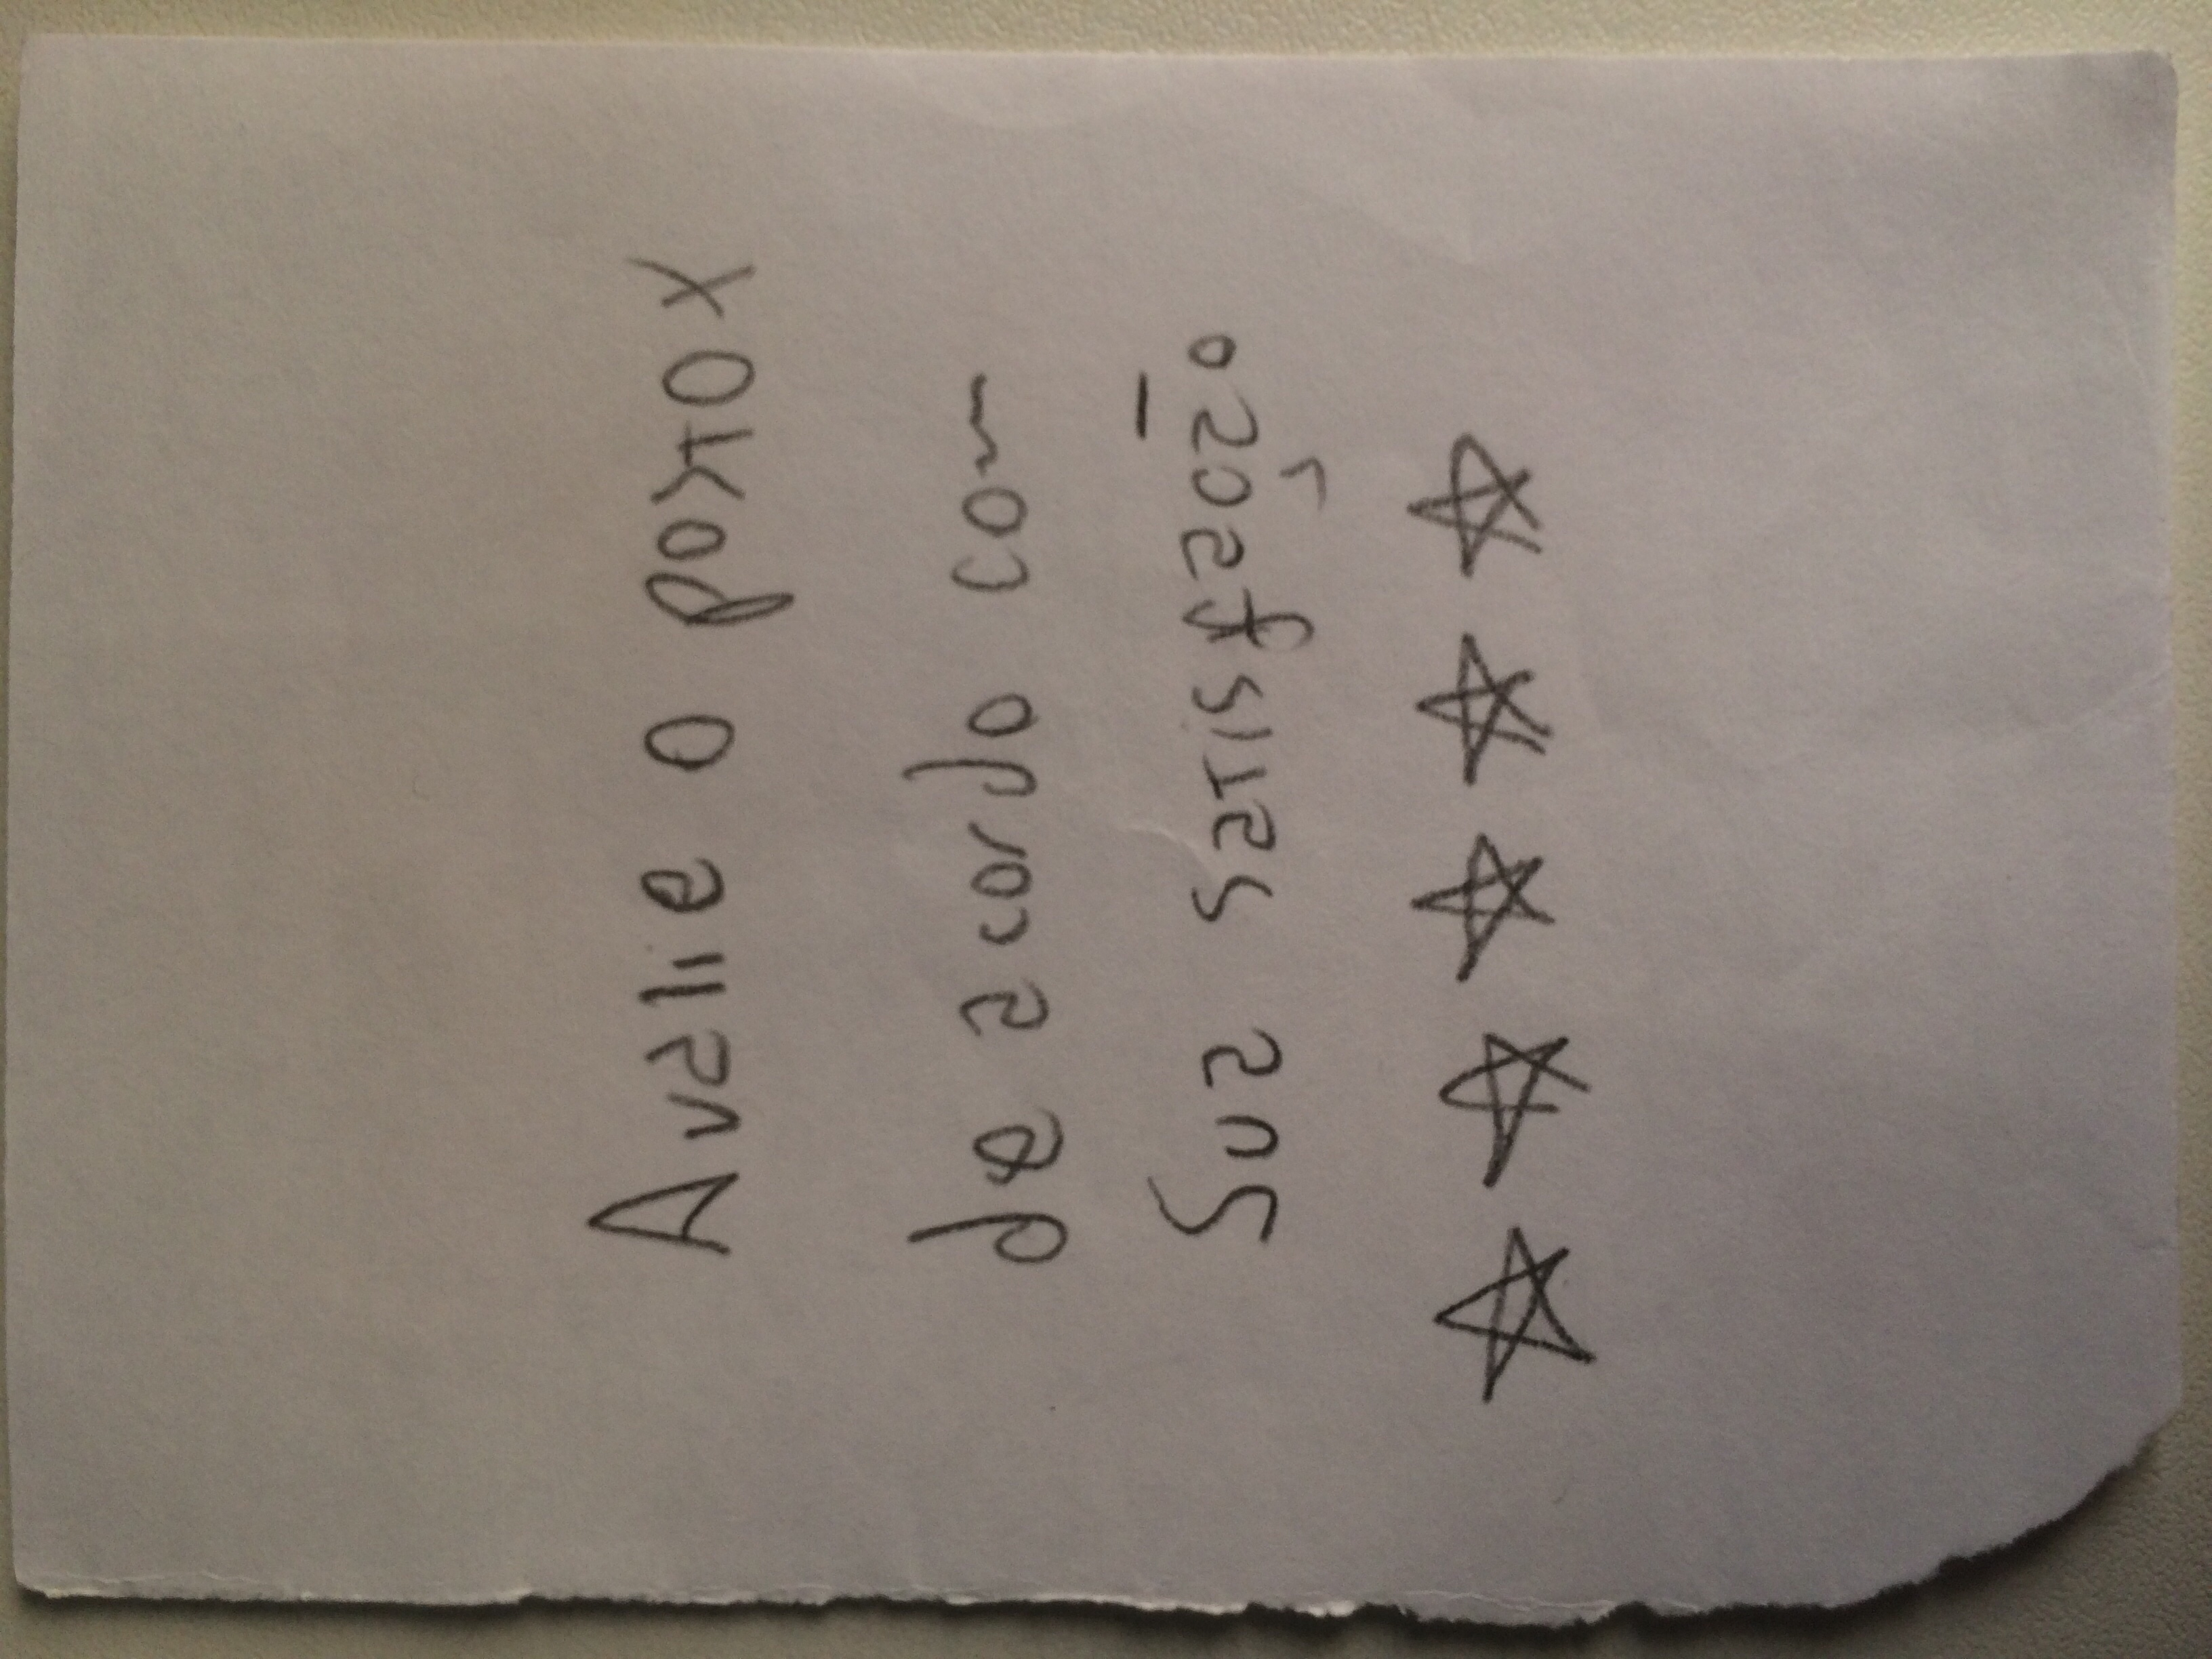
\includegraphics[scale=0.1, angle=-90]{figuras/prototipo_papel_avaliar_posto.jpg}
    \caption[Protótipo de papel da tela de avaliar um posto de combustíveis]{Protótipo de papel da tela de avaliar um posto de combustíveis. Fonte: autores}
    \label{img:prototipo_de_papel_avaliar_posto}
\end{figure}
 \pagebreak

A Figura \ref{img:prototipo_de_papel_postos_boicotados} mostra o protótipo de papel da tela com uma lista de postos boicotados.
\begin{figure}[H]
    \centering
    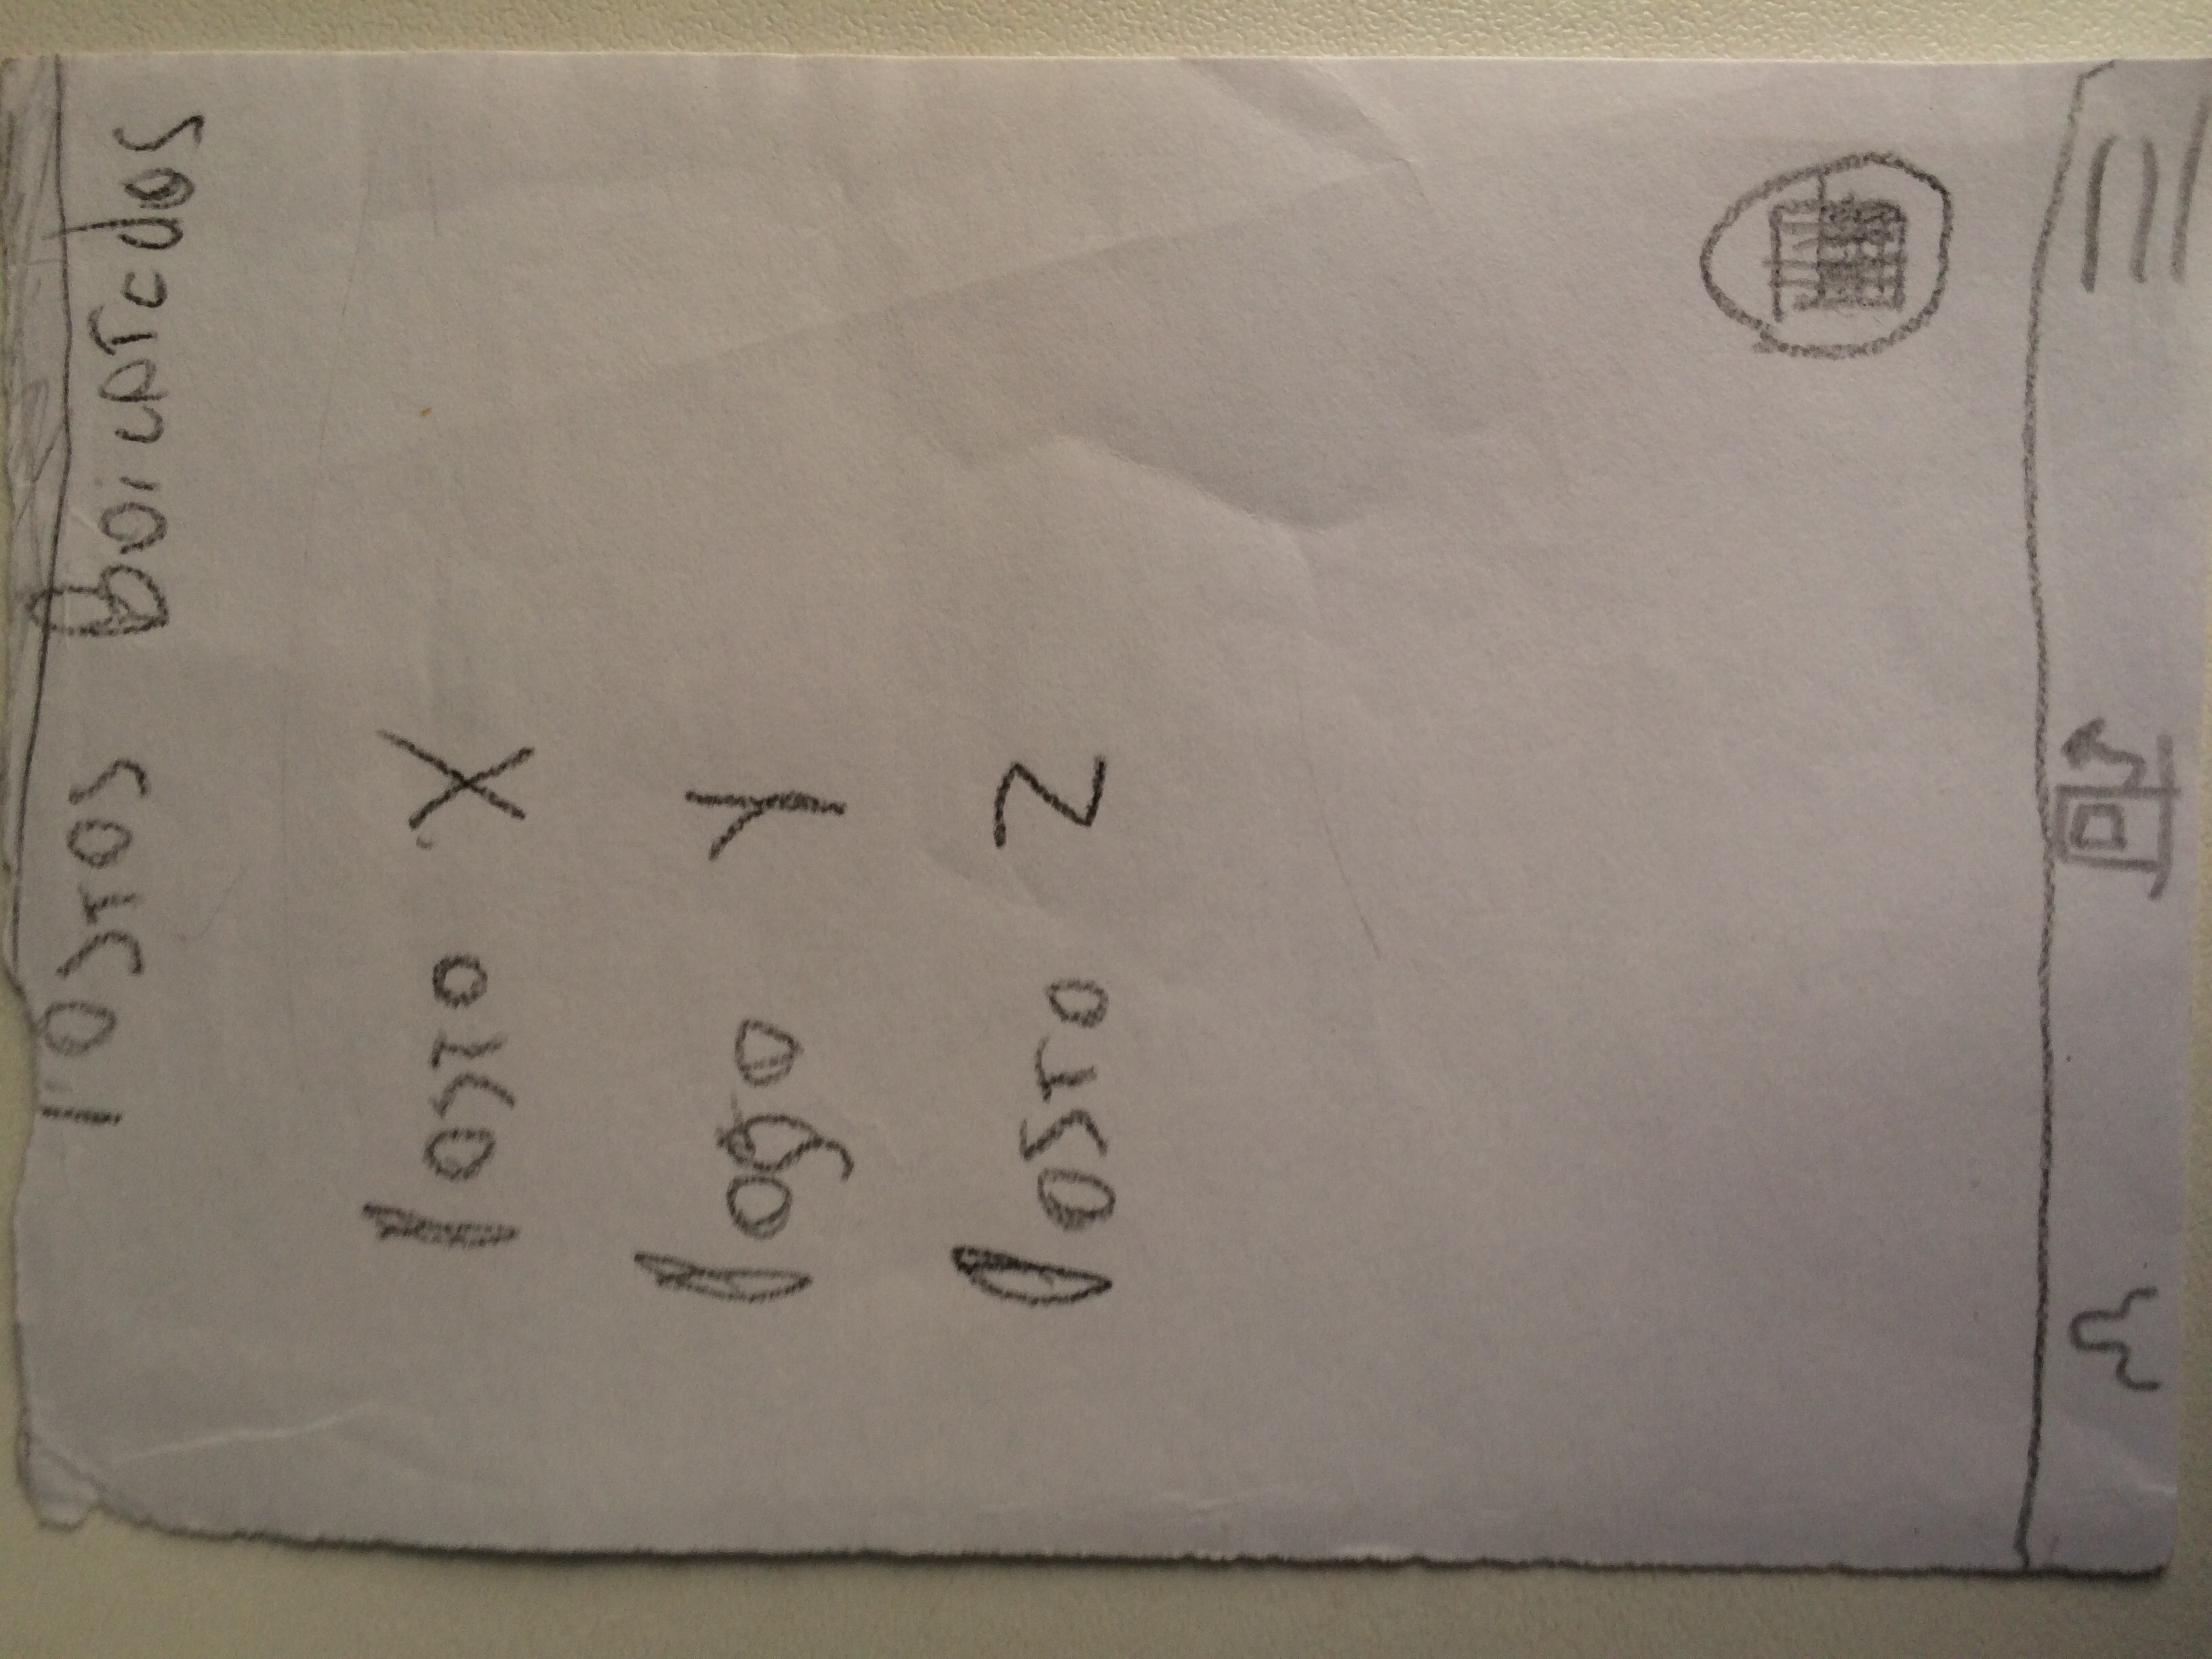
\includegraphics[scale=0.1, angle=-90]{figuras/prototipo_papel_postos_boicotados.jpg}
    \caption[Protótipo de papel da tela de postos boicotados]{Protótipo de papel da tela de postos boicotados. Fonte: autores}
    \label{img:prototipo_de_papel_postos_boicotados}
\end{figure}
 \pagebreak

A Figura \ref{img:prototipo_de_papel_lista_postos} mostra o protótipo de papel da lista de postos de combustíveis. Que a priori pode ser ordenada por preço e distância.
\begin{figure}[H]
    \centering
    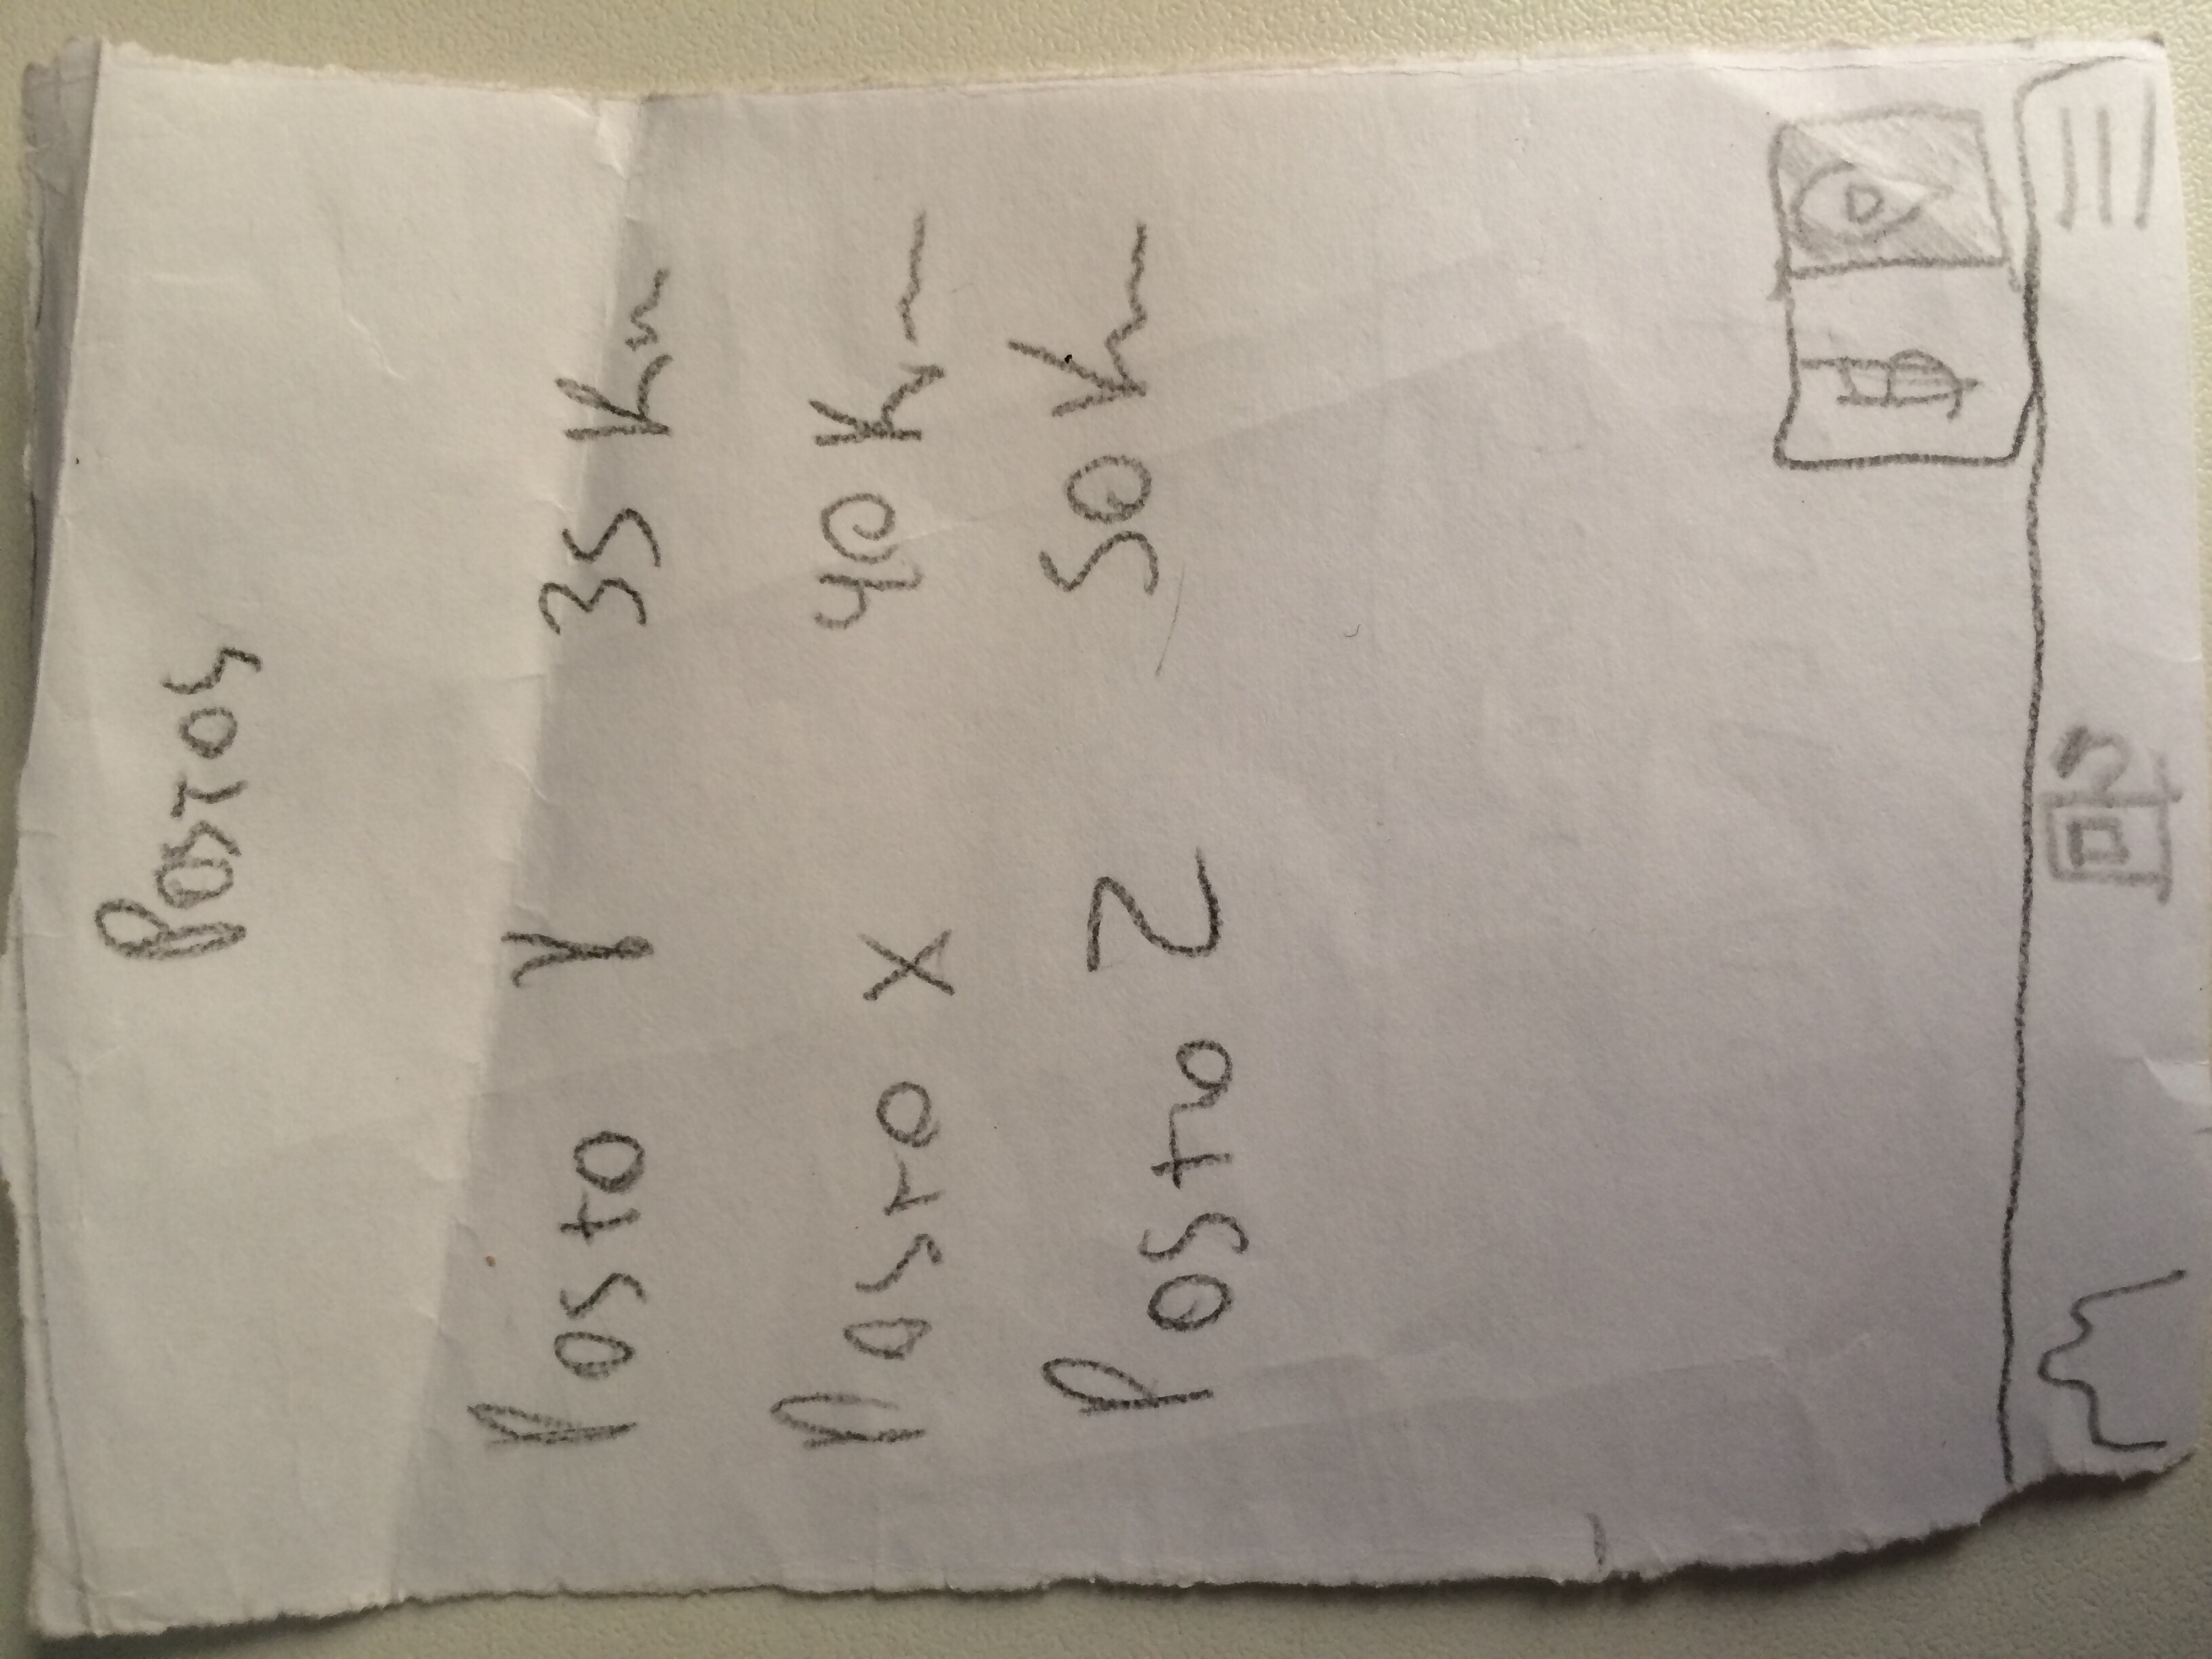
\includegraphics[scale=0.1, angle=-90]{figuras/prototipo_papel_lista_de_postos.jpg}
    \caption[Protótipo de papel da tela de postos de combustíveis]{Protótipo de papel da tela de postos de combustíveis. Fonte: autores}
    \label{img:prototipo_de_papel_lista_postos}
\end{figure}
 \pagebreak

A Figura \ref{img:prototipo_de_papel_marvel} mostra as 8 telas sendo utilizadas no aplicativo Marvel, para a simular a interação entre telas.
\begin{figure}[H]
    \centering
    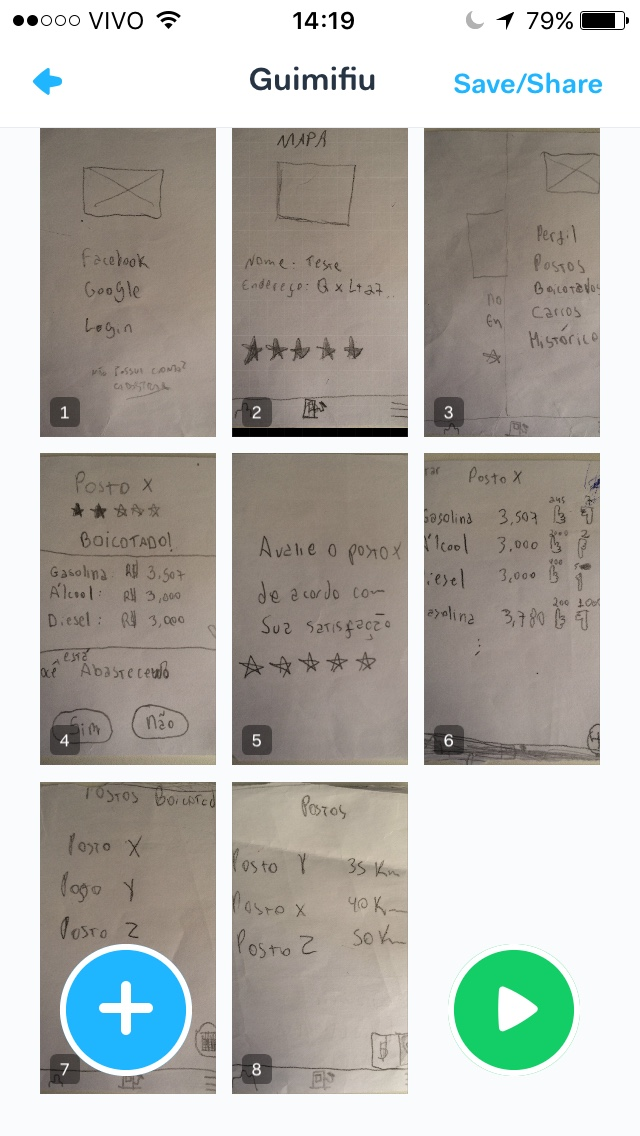
\includegraphics[scale=0.3]{figuras/prototipo_de_paple_marvel.jpg}
    \caption[Protótipos de papel utilizados no aplicativo Marvel]{Protótipos de papel utilizados no aplicativo Marvel. Fonte: autores}
    \label{img:prototipo_de_papel_marvel}
\end{figure}
 \pagebreak

A Figura \ref{img:prototipo_tela_de_login} mostra o protótipo da tela de login da aplicação. O login pode ser feito via Facebook, Google ou criando uma conta local.
\begin{figure}[H]
    \centering
    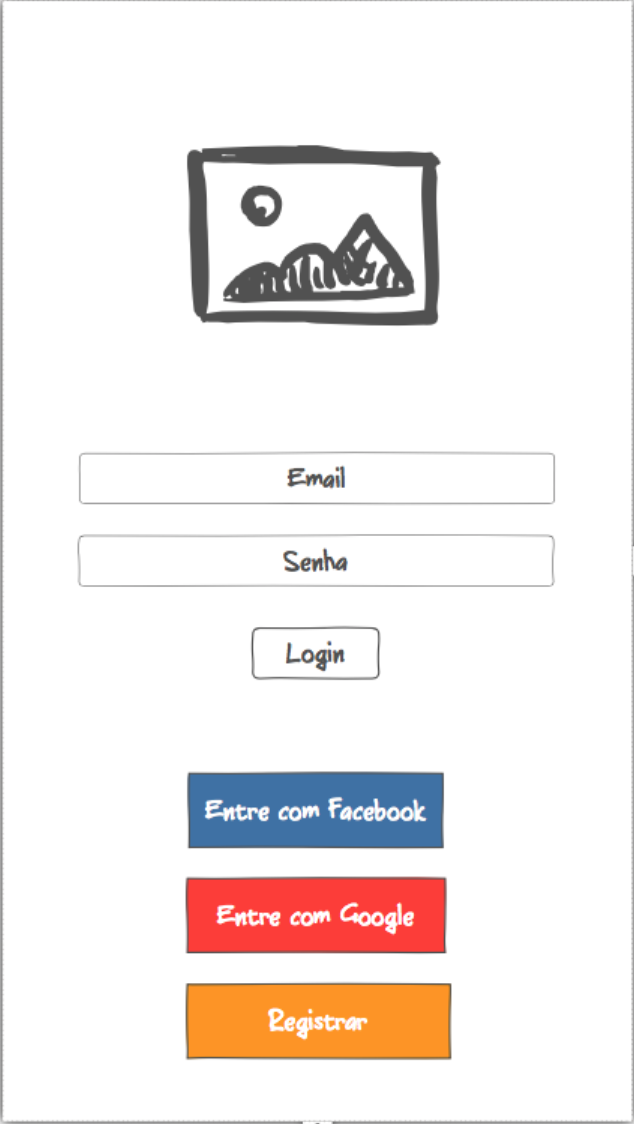
\includegraphics[scale=0.5]{figuras/prototipo_login.png}
    \caption[Protótipo da tela de login]{Protótipo da tela de login. Fonte: autores}
    \label{img:prototipo_tela_de_login}
\end{figure}
 \pagebreak

A Figura \ref{img:prototipo_tela_de_cadastro} mostra o protótipo da tela de cadastro da aplicação.
\begin{figure}[H]
    \centering
    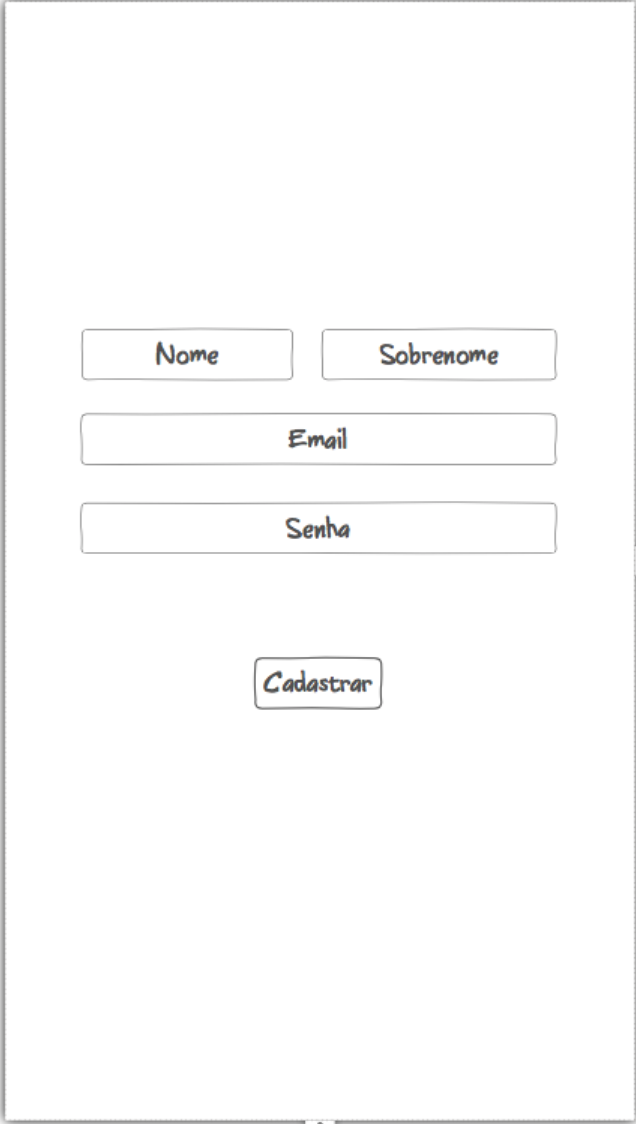
\includegraphics[scale=0.5]{figuras/prototipo_cadastro.png}
    \caption[Protótipo da tela de cadastro]{Protótipo da tela de cadastro. Fonte: autores}
    \label{img:prototipo_tela_de_cadastro}
\end{figure}
 \pagebreak
A Figura \ref{img:prototipo_tela_inicial} mostra o protótipo da tela inicial da aplicação, que mostra o mapa para usuário navegar e visualisar postos de combustíveis.

\begin{figure}[H]
    \centering
    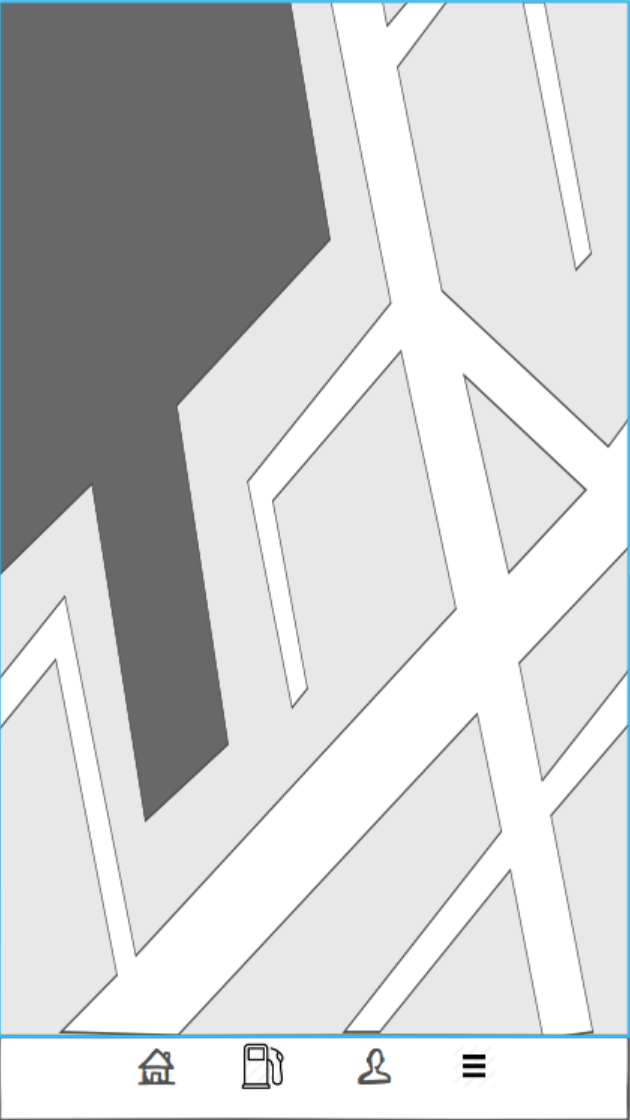
\includegraphics[scale=0.5]{figuras/prototipo_mapa.png}
    \caption[Protótipo da tela inicial]{Protótipo da tela inicial. Fonte: autores}
    \label{img:prototipo_tela_inicial}
\end{figure}
